\documentclass{article}
    \usepackage{graphicx}
    \usepackage[absolute,overlay]{textpos}
    \setlength{\TPHorizModule}{1mm}
    \setlength{\TPVertModule}{1mm}
    \date{}
    \title{Elliott's Games!}
    \begin{document}
    \maketitle
    \centering
    \begin{textblock}{50}(-5,0)
    \rotatebox{45}{\includegraphics[width=25mm]{/Users/elliottmacneil/python/reti/data/animals/stoat1.jpg}}
    \end{textblock}
    Today's set of puzzles are mostly taken from the 2021 Online London Chess League, and a couple from the 2000 Bundesliga in Germany.
    Once again, if you get stuck, ask one of the coaches to come and help! Write your solutions \textbf{in notation}. 
    \newline
    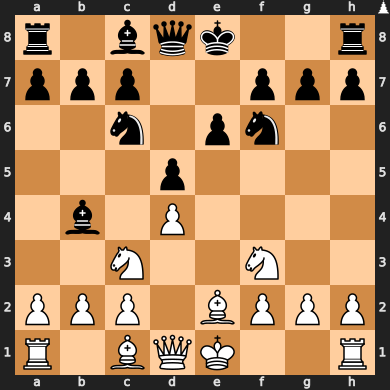
\includegraphics[width=6cm, height=6cm]{/Users/elliottmacneil/python/reti/notebooks/exploratory/puzzles/8.png}
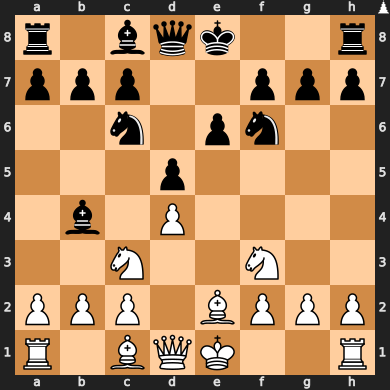
\includegraphics[width=6cm, height=6cm]{/Users/elliottmacneil/python/reti/notebooks/exploratory/puzzles/9.png}
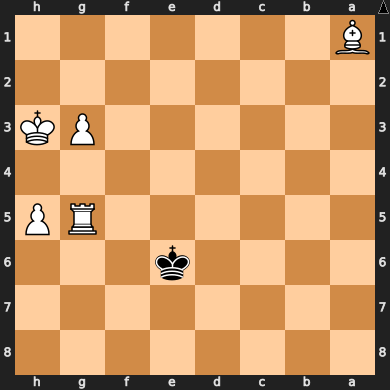
\includegraphics[width=6cm, height=6cm]{/Users/elliottmacneil/python/reti/notebooks/exploratory/puzzles/12.png}
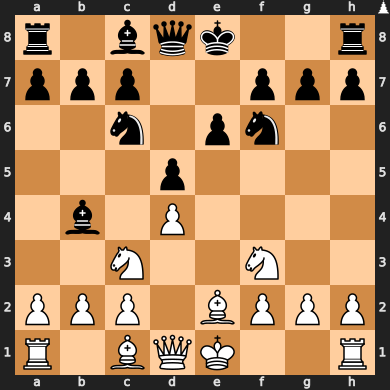
\includegraphics[width=6cm, height=6cm]{/Users/elliottmacneil/python/reti/notebooks/exploratory/puzzles/13.png}
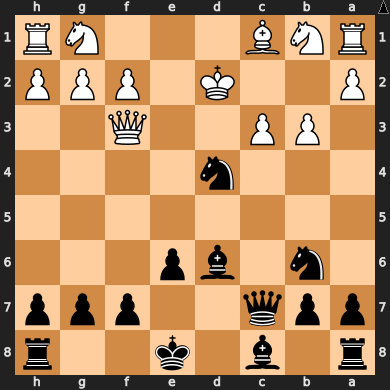
\includegraphics[width=6cm, height=6cm]{/Users/elliottmacneil/python/reti/notebooks/exploratory/puzzles/11.png}
\end{document}